\documentclass{school-22.101-notes}
\date{December 14, 2011}

\begin{document}
\maketitle


\lecture{Final Review}

\topic{Introduction}
Z-related terms: 
\begin{enumerate}
\item CGS unit: $\hbar c = 200 \fsp \MeV \cdot \fm$; the fine structure constant $\frac{e^2}{\hbar c} = \frac{1}{137}, m_n c^2 = 938.$
\item Calculate energy:
\eqn{ E_{\mathrm{ISW}} = \frac{Z_1 Z_2 e^2}{r^2} = \frac{Z_1 Z_2}{r^2} (\hbar c) \frac{e^2}{\hbar c} }
\item $mc^2$ for proton/neutron is about 940 MeV; electron is 0.5 MeV; reduced mass is $\frac{m_1 m_2}{m_1 + m_2}$. 
\eqn{ \frac{\hbar^2 \pi^2}{2 m L^2} = \frac{(\hbar c)^2 \pi^2}{2 (mc^2) L^2}   }
\item Alpha decay:
\eqn{ E_G = \left(\frac{2 \pi e^2 Z_{\alpha} Z_D}{\hbar c}\right)^2 \frac{\mu c^2}{2} = \left( \frac{2 \pi \cdot Z_{\alpha} Z_D}{137} \right)^2 \frac{m_{\alpha} m_D}{m_{\alpha} + m_D} \frac{938}{2} }
\end{enumerate}

Stuffs should know on top of head: 
\begin{enumerate}
\item R (in F)$ = (1.2 \sim 1.4) A^{1/3}.$
\end{enumerate}


Math: 
\eqn{ \sin^2(kx) = \frac{1}{2} \left[ 1 - \cos (2kx) \right] }
\eqn{ \cos(kx) &= \mathrm{Re}(e^{ix}) = \frac{e^{ikx} + e^{-ikx}}{2} &  \sin(kx) &= \mathrm{Im}(e^{ix}) = \frac{e^{ikx} - e^{-ikx}}{2i} }
Integration by parts: 




%%%%%%%%%%%%%%%%%%%%%%%%% Topic 1 Quantum Mechanics %%%%%%%%%%%%%%%%%%%%%%%%%%%%
\clearpage
\topic{Solve Schrodinger Equation}
\begin{enumerate}
\item TISE: 
  \begin{align}
    \hat{H} \psi_n  &= E_n \psi_n  & 
    - \frac{\hbar^2}{2m} \dpsidxn2 + V \psi_n  &= E_n \psi_n  & - \frac{\hbar^2}{2m} \dpsidxn2   &= (E_n - V) \psi_n  
\end{align}
\begin{align}
\begin{dcases*}
\dpsidxn2 = - k^2 \psi_n, \fsp k = \sqrt{\frac{2 m (E - V)}{\hbar^2}} & Allow region, $E > V$. \\
\dpsidxn2 = \kappa^2 \psi_n, \fsp \kappa = \sqrt{\frac{2 m (V - E)}{\hbar^2}} & Forbidden region, $E < V$. 
\end{dcases*}
  \end{align}


  
\item Normalization:
\begin{align}
\int_{-\infty}^{\infty} |\psi(x)|^2 \dx &= 1 \\
\int_0^{\infty} 4 \pi r^2 \dr |\psi(r)|^2 &= 1 \\
\int_0^{2 \pi} \dpsi \int_0^{\pi} \sin \theta \dtheta |Y(\theta, \psi)|^2 &= 1 
\end{align}

\item Expectation: $ \expect{A} = \int_{-\infty}^{\infty} \psi^* A \psi \dx $.

\item Decompose wave function into bases: 
\begin{align}
\psi(x) &= \Sum_{n=1}^{\infty} C_n w_n (x) & \psi (x,t) &= \Sum_{n=1}^{\infty} C_n w_n(x) e^{ \frac{-iE_nt}{\hbar} } \\
P_n &= P(E_n) = |C_n|^2  & C_n &= \int w_n^* (x) \psi(x) \dx = \braket{w_n}{\psi}
\end{align}

\item Ehrefest theory: $ \ddt \expect{A} = \frac{i}{\hbar} \expect{\left[ \Hhat, \Ahat \right] } + \overbrace{\expect{\ddt \Ahat}}^{\to 0} $. Application: $\ddt \expect{x} = \frac{1}{m} \expect{p}$. 

\item 

\begin{table}[h]
  \centering 
  \begin{tabular}{|c|c|c|c|} \hline
    Observable & Operator & Eigenvalue & Eigenfunction \\ \hline
    Position & $\hat{x} = x$ & $x_0$ (any $x_0$) & $\delta (x - x_0)$ \\ \hline
    Momentum & $\hat{p} = - i \hbar \nabla$ & $p = \hbar k$ (any $k$) & $u_n = A e^{ikx}$ \\ \hline
    Energy & $\hat{H} = \frac{\hat{p}^2}{2m} + V(x) = - \frac{\hbar^2}{2m} \laplacian + V(x)$ & ? & ? \\ \hline
  \end{tabular}
  \caption{Operator Eigenvalue and Eigenfunction}
\end{table}

\begin{itemize}
\item Position space: $\hat{p} = -i\hbar \ddx, \hat{H} = - \frac{\hbar^2}{2m} \nabla^2 + V(x) = \frac{\hat{p}^2}{2m} + V(x)$. 
\item Phase space: $\phat = \hbar k, \expect{E_n} = \frac{\hbar^2 k^2}{2m}$. 
\end{itemize}

\item Commutation of operators:  
\begin{align}
[\hat{x}, \hat{p} ] &= i \hbar & [\hat{L}^2, \hat{H} ] &= 0 \\
[ \hat{x}, \hat{p}^2] &= [\hat{x}, \hat{p} ] \hat{p} + \hat{p} [\hat{x}, \hat{p} ]  = 2 i \hbar \hat{p} & [\hat{x}^2, \hat{p} ] &= \hat{x} [\hat{x}, \hat{p} ] + [\hat{x}, \hat{p} ] \hat{x} = 2 i \hbar \hat{x} \\
\ddt \expect{\hat{x}} &= \frac{\expect{\hat{p}}}{m} & \ddt \expect{\hat{p}} &= - \expect{ \dVdx }
\end{align}
Two operator commute (they have common eigenvectors, can measure both at the same time) if and only if $[A, B] = 0$. 

\item Fourier transform between position space and momentum space:
\eqn{ \phi(k) = \frac{1}{\sqrt{2\pi}} \int_{-\infty}^{\infty} e^{-ikx} \psi (x) \dx }
\eqn{ \phi(x) = \frac{1}{\sqrt{2\pi}} \int_{-\infty}^{\infty} e^{ikx} \psi (k) \dk }
\eqn{ \delta(x - \alpha) = \frac{1}{2\pi} \int_{-\infty}^{\infty} e^{ip(x-\alpha)} \derivative p }


\item Common potentials: notice, $e^{ikx}$ means traveling to the right, $e^{-ikx}$ means traveling to the left ($e^{-\kappa x}$ is decaying to the right, $e^{\kappa x}$ is reflecting back to the left). For calculating $T, R$, we do the ratio of flux, which is defined as: $\Gamma = |\psi|^2 \frac{\hbar k}{m}$. See HW2 \#2.
\begin{table}[ht]
    \centering
    \begin{tabular}{|p{1.4in}|c|c|c|} \hline
    Potential & Allowed energies & Wave forms & Wave bases\\ \hline
    ISW/Particle in a box & $E_n = \frac{n^2 \pi^2 \hbar^2}{2 m a^2} $ &  & $\psi_n (x) = \sqrt{\frac{2}{a}} \sin \left( \frac{n \pi x}{a} \right) $ \\ \hline
    \multirow{2}{*}{FSW} &  & $\psi(x) = A e^{ikx} + B e^{-ikx}, k = \frac{\sqrt{2m(E-V_1)}}{\hbar} $ & \\ 
     &  & $\psi(x) = C e^{\kappa x} + D e^{-\kappa x}, \kappa = \frac{\sqrt{2m(V_2 - E)}}{\hbar} $ & \\ \hline    
    Step Barrier, if $E>V$ & & $A e^{ik_1 x} + B e^{-ik_1 x}, Ce^{ik_2x} $   & \\ \hline
    Step Barrier, if $E<V$ & & $A e^{ik_1 x} + Be^{-ik_1 x}, C e^{-\kappa x}$ & \\ \hline
    Rectanger Step Barrier & & $A e^{i k_1 x} + B e^{-ik_1 x}, Ce^{\kappa x} + D e^{-\kappa x}, E e^{ik_1 x}$ & \\ \hline
    \end{tabular}
    \caption{Common Potentials}
\end{table}

\item Drawing wavefunction. Example: HW2 \#3. 
\begin{itemize}
\item Frequency/wavelength is related to KE $ = E - V$: the smaller KE is, the tighter the wavefunctions are. 
\item Amplitude is related to the change in potential: every time potential changes (whether increase or decrease), amplitude decreases. If the potential does a jump change, amplitude just decreases; if the potential gradually decreases, then amplitude graduate decreases as well. 
\end{itemize}

  \begin{figure}[h]
    \centering
    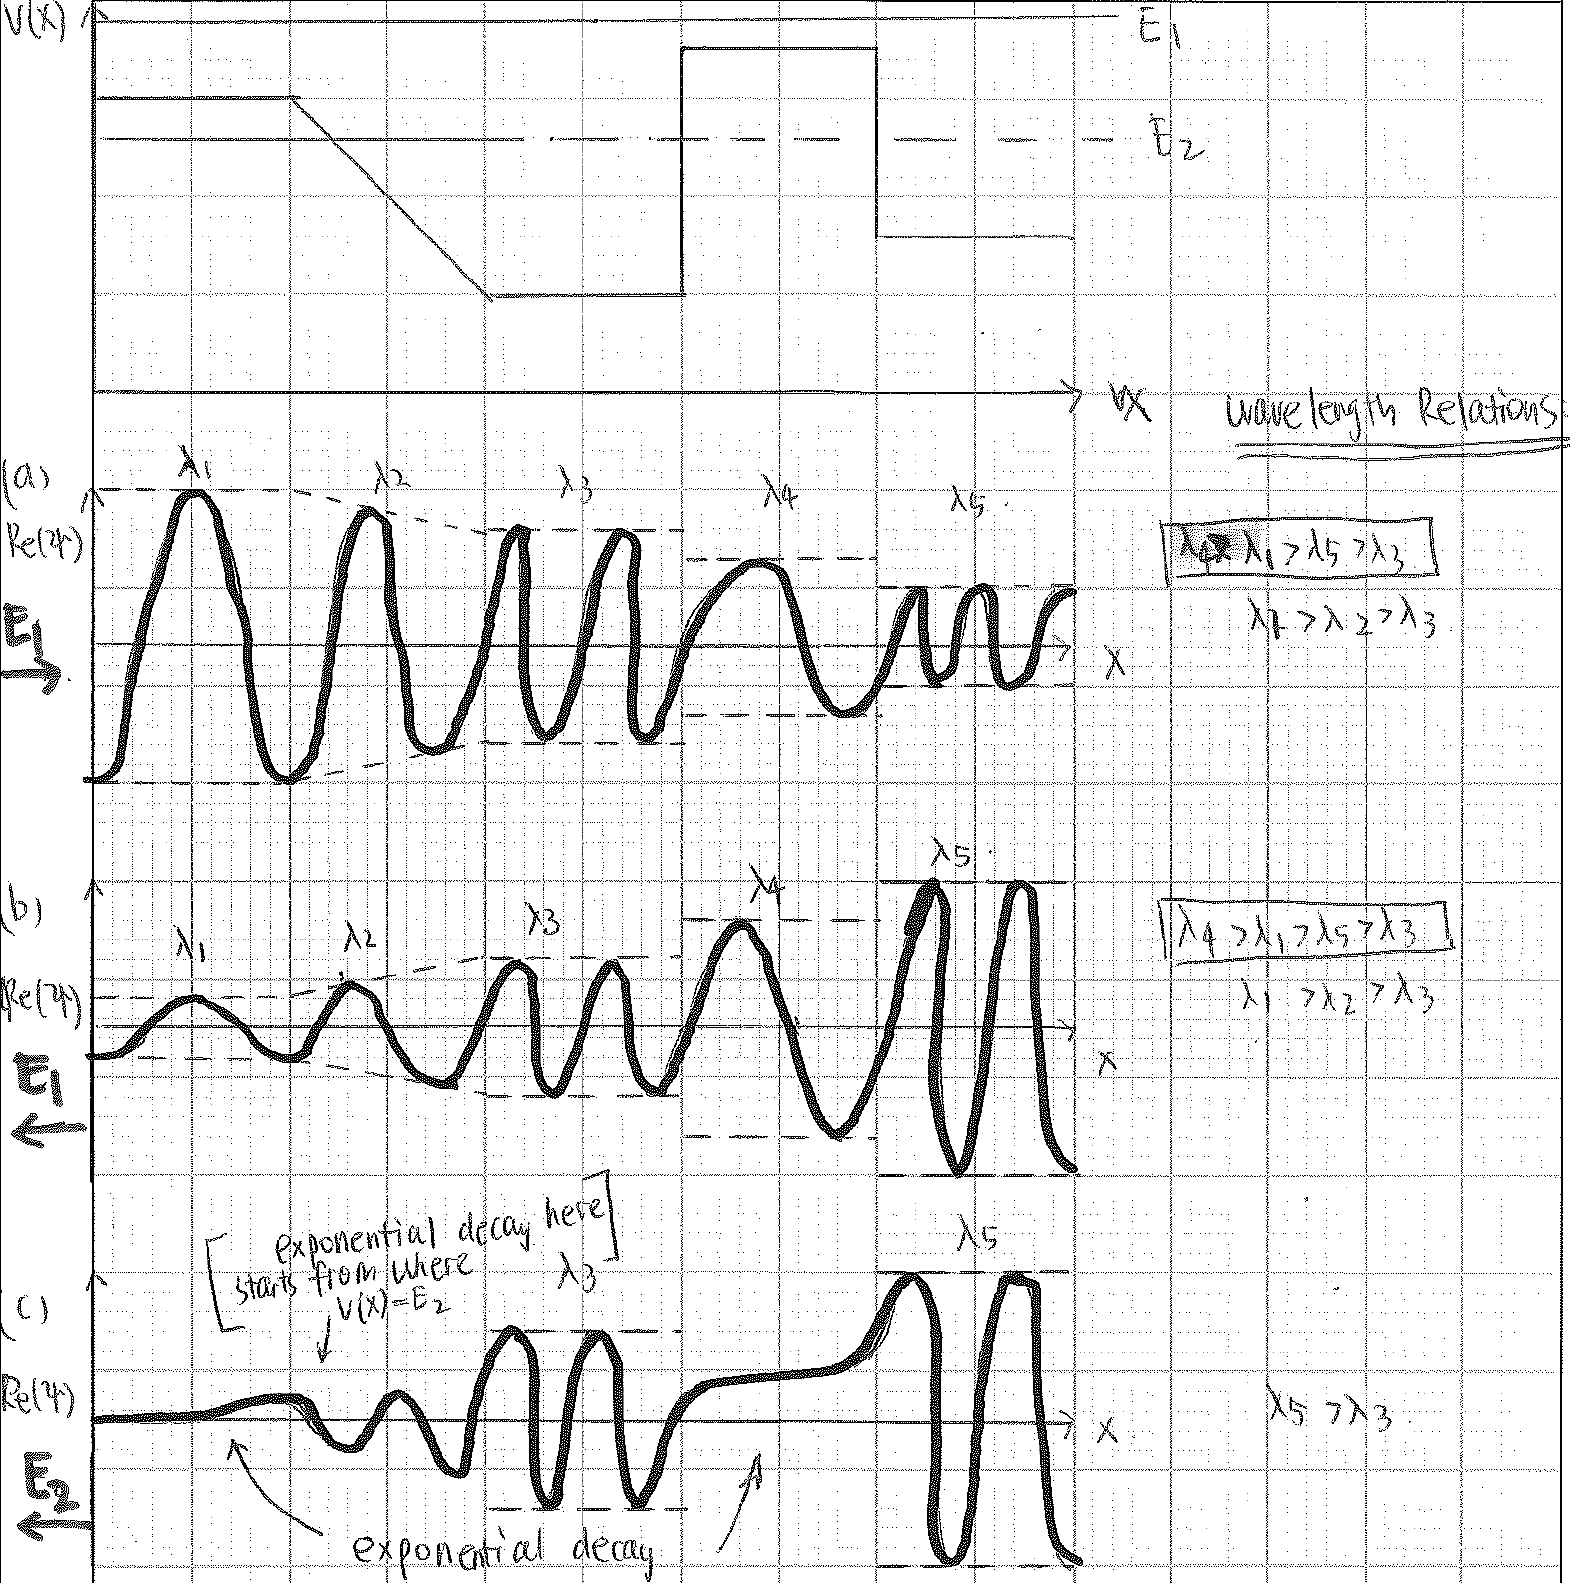
\includegraphics[width=4in]{../HW/HW2/images/HW2-3-graph.png}
  \end{figure}

\item TDSE: 


\item Compute period: 2011 HW3 \#4(i). 2012 HW3 \#6(f). If no common factor among allowed $n$'s, then $T = \frac{2 \pi \hbar}{E_1}$. If $\psi$ is a polynomial, then infinite $n$'s, thus period is the above again.  
\end{enumerate}



\end{document}





